\section{Однолучевые алгоритмы оценки угла прихода сигнала в системе 5G NR}
\label{sec:singlepath}
\subsection{Иерархический поиск}
Эффективность иерархического поиска, в результатах симуляции в разделе
\ref{sec:simulations} он назван \textit{baseline}, рассматривается как нижняя
граница разработанных алгоритмов.  Можно было бы в качестве базового алгоритма рассматривать
метод Фурье (см. \ref{sec:fourier}) и необходимый для него полный перебор
по всем парам лучей (UE-BS), примененный к меняющемуся во времени каналу.
Однако он дает слишком высокую ошибку дискретизации и сравнивать с ним
результаты других алгоритмов оказалось не наглядно.

Алгоритм состоит из двух этапов: полного перебора всех пар лучей UE-BS и
процедуры дополнительных измерений.
На первом этапе пользователь использует ортогональную кодовую книгу, покрывающую
диапазон углов от $-\pi$ до $\pi$:
\begin{equation}
    \vec w_u =
    \begin{bmatrix}
        1 & \exp {i \eta_u} & \dots & \exp{i(N-1)\eta_u},
    \end{bmatrix}^T
\end{equation}
\begin{equation}
    \eta_u = -\pi \frac{N-1}{N} + 2\pi \frac{u-1}{N},
\end{equation}
где $N$ -- число элементов антеннйо решетки, $u$ -- индекс весового вектора, лежащий в интервале $\qty[1 \dots N]$, $\eta_u$ -- обобщенный угол, соответствующий углу прихода сигнала следующим образом
\begin{equation}
    \eta_u = 2\pi \frac{d}{\lambda_w}\sin\phi_u,
\end{equation}
где $d$ -- расстояние между элементами решетки, $\lambda_w$ -- длина волны. ДН,
получаемые с помощью данной кодовой книги показаны на рис. \ref{fig:4.9}
сплошными линиями.
\begin{figure}[ht]
    \centering
    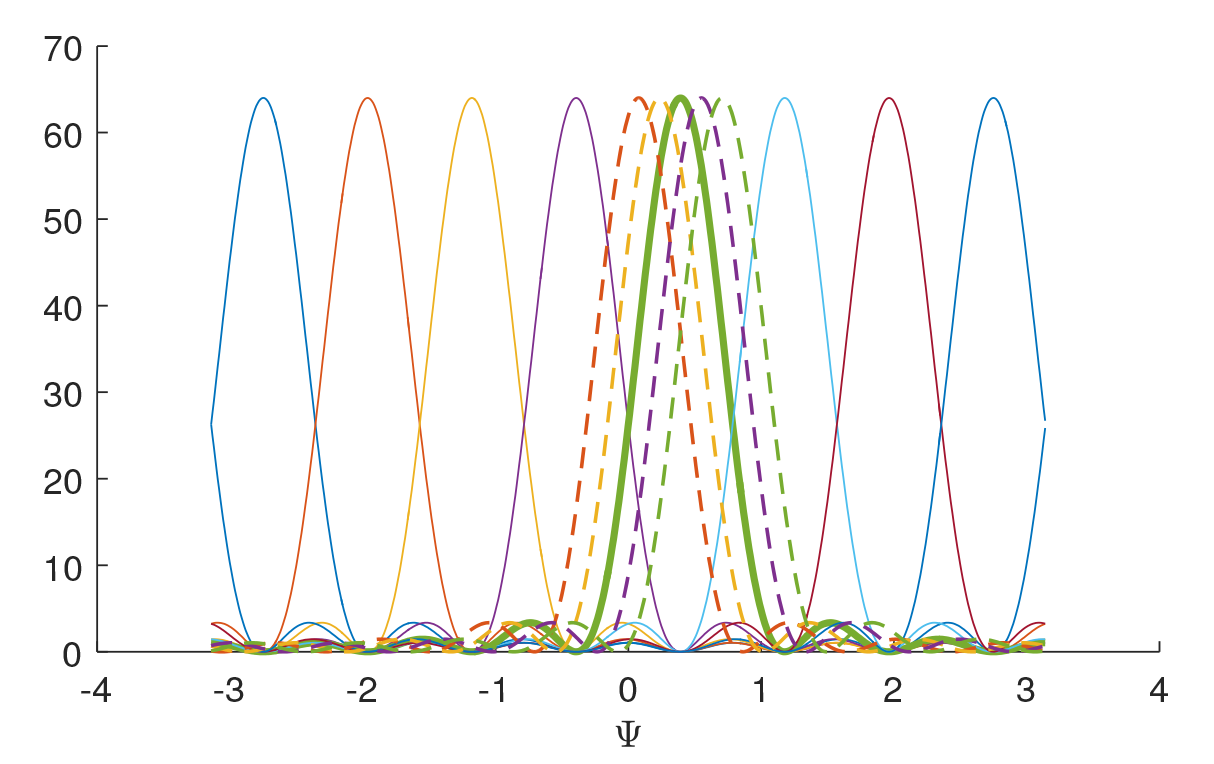
\includegraphics[width=0.5\linewidth]{figs/fig4.8}
    \caption{Различные ДН, формируемые кодовой книгой на стороне пользователя. $\psi$ -- обобщенный угол, $N=8$, $M=4$}
    \label{fig:4.9}
\end{figure}

Пусть $v$ -- индекс наилучшего весового вектора $\vec w_u^{(v)}$, который
обеспечивает наибольшую принятую мощность на антенной решетке.  Соответствующая
ДН показана на рис. \ref{fig:4.9} толстой сплошной линией. Пусть $p_v$ --
мощность, измеренная для вектора $\vec w_u^{(v)}$. На этапе дополнительных измерений
пользователь тестирует $M$ дополнительных весовых векторов, чтобы уменьшить
ошибку дискретизации.
\begin{equation}
    \label{eq:4.19}
    \vec w_q =
    \begin{bmatrix}
        1 & \exp {i \chi_q} & \dots & \exp{i(N-1)\chi_q},
    \end{bmatrix}^T
\end{equation}
\begin{equation}
    \chi_q = \eta_v + 2\pi \frac{q}{N(M+1)},
\end{equation}
где $q=-0.5M,\dots,-1,+1,\dots,+0.5M$. Сформированные дополнительные ДН показаны
на рис.\ref{fig:4.9} пунктирными линиями.  Обозначим $p_0= p_v$ и $\chi_0 =
    \eta_v$. Отметим, что для процедуры уточнения не нужно проводить измерения
$\chi_0$, поскольку оно уже было сделано на предыдущем этапе.  Наонец, путь
распространения с обобщенным углом $\hat \psi$ оценивается как один из $\chi_q
    \in \qty{\chi_{-0.5 M}, \dots, \chi_0, \dots, \chi_{+0.5M}}$, обеспечивающий
наибольшую измеренную мощность $p_q$. Угол прихода соответствующего луча
оценивается как
\begin{equation}
    \hat \phi = \arcsin{\frac{\psi \lambda_w}{2\pi d}}.
\end{equation}

Процедура измерения алгоритма представлена на рис. \ref{fig:4.10} и происходит следующим образом:

\begin{enumerate}
    \item Sector Level Sweep Stage. BS periodically sweeps its beams. UE
          sequentially uses each beam of codebook (4.16) to measure power for each
          beam of BS. This procedure is performed for AIP1 and AIP2
    \item We choose the best UE-BS beam pair and consider the selected UE’s
          beam as the best sector with spatial frequency $\eta_v$.
    \item Refinement procedure stage. BS periodically sweeps its beams. UE
          sequentially uses each beam of codebook (4.19) to measure power for each
          beam of BS.
    \item We choose the best UE-BS beam pair among all measured at step 3 and
          measured for the central beam of the best sector at step 1. The spatial
          frequency of the selected UE’s beam is $\hat \psi$.
          %  \item If the best UE-BS beam pair is related to AIP1, $\hat \phi_{AOA} = \hat \phi$ 
          %  determined in (4.21).  If the best UE-BS pair is related to AIP2, φ ̂_AOA=φ
          %  ̂+ π. The result is obtained in radians.
\end{enumerate}

\begin{figure}[ht]
    \centering
    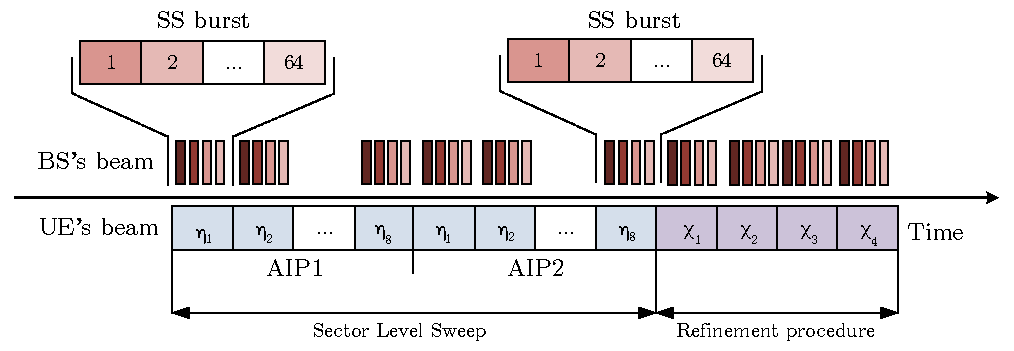
\includegraphics[width=\linewidth]{figs/fig4.9}
    \caption{Изображение процедуры иерархического поиска (\textit{baseline}) во времени для двух антенных решеток. $N=8$, $M=4$, 64 луча BS}
    \label{fig:4.9}
\end{figure}

Параметры алгоритма иерархического поиска представлены в таблице \ref{tab:4.2}.
Предполагается, что один SS-burst состоит из 64 RS и занимает 32 последовательных слота с периодом 20 мс.

\begin{table}
    \caption{Параметры алгоритма иерархического поиска (baseline)}
    \label{tab:4.2}
\end{table}


\subsection{Иерархический поиск с минимизацией СКО}
В теории оценивания AOA доказано, что наилучшее решение дает максимально правдоподобная оценка (Maximum Likelihood Estimator).
Рассматривая случай однолучевого канала, можно представить уравнение \eqref{eq:3.10} в виде
\begin{equation}
    d(\phi) = \sum\limits_q \vec y^H(q) \vec y(q) - \sum\limits_q\abs{\vec y^H \vec s(\phi)}^2 \to \min_\phi,
\end{equation}
\begin{equation}
    \label{eq:4.23}
    \sum\limits_q \abs{\vec y^H(q) \vec s(\phi)}^2 = \hat p(\phi) \to \max_\phi,
\end{equation}
где $\vec y$ -- вектор принятого антенной решеткой сигнала, $\vec s(\phi)$ --
фазирующий вектор. Выражение \eqref{eq:4.23} имеет смысл мощности,
принимаемой с  вектором $\vec s(\phi)$, обеспечивающим максимум ДН в направлении
$\phi$. Максимизация этого значения есть ни что иное, как непрерывное
сканирование лучом и получение пространственного распределения мощности.

На практике, мы не можем применить этот оптимальный алгоритм по нескольким
причинам. Во-первых, мы \hl{управляем лучами дискретными фазовращателями и можем
    оценить только дискретный спектр мощности}. Разумеется, можно применить некоторые
методы интерполяции, но это будет только приближение.  Во-вторых, у нас есть
сильные ограничения по времени, особенно в случае динамического канала.  Таким
образом, метод иерархического поиска, который адаптивно измеряет дискретный
спектр мощности, представляется наиболее подходящей аппроксимацией оптимального
МП-оценки.

Однако, приближение спектра мощности с помощью иерархического
поиска, каким он рассматривался в предыдущем разделе \eqref{sec:hierarchy}, не
является удачной аппроксимацией.  Прежде всего потому что это приближение с
ошибкой дискретизации. К тому же, если искомая угловая координата источника
лежит на стыке  двух антенных решеток $\hat \phi \approx \pm \pi$ или же просто
при низком SNR,  можно ошибиться с выбором антенной решетки и эта ошибка не
будет исправлена в дальнейшем. С учетом этим недостатков, был разработан
улучшенный алгоритм иерархического поиска.


На первый взгляд, проблема дискретизации может быть решена с помощью
МП-оценки, адаптированного к последовательному измерению отклика мощности
луча. Однако полученная в этом случае функция правдоподобия сложна для анализа
(здесь предполагается, что амплитуда принимаемого сигнала имеет распределение
Райса).

\begin{equation}
    F_{ML}(\psi, a) = \prod\limits_m \frac{1}{\sigma^2}
    \exp{-\frac{\hat p_m + a f_m(\psi)}{\sigma^2}
        I_0\qty(\frac{2\sqrt{\hat p_m a f_m(\psi)}}{\sigma^2})} \to \max_{\psi, a},
\end{equation}
где $\hat p_m$ -- измеренная мощность на $m$-ом луче, $\sigma^2$ -- мощность
шума, $a$ -- "мощность" некоторого путя распространения, $I_0(x)$ --
модицицированная функция Бесселя, $f_m(\psi)$ -- усиление АР для $m$-го луча в
направлении обобщенного угла $\chi_m$, $\psi = 2\pi \frac{d}{\lambda_w}\sin
    \phi$ -- обобщенный угол, а $\phi$ -- угол прихода.
\begin{equation}
    f_m(\psi) = \frac{\sin^2 (0.5N(\psi - \chi_m))}{\sin^2(0.5(\psi - \chi_m))}.
\end{equation}
Поскольку мы пытаемся найти простое решение, мы предлагаем взять в основу
критерий минимума СКО, вместо МП-оценки.
\begin{equation}
    \label{eq:26}
    F_{MMSE}(\psi, a) = \sum\limits_m \qty(\hat p_m - a f_m(\psi))^2 \to \min_{\psi,a}
\end{equation}

В первую очередь, необходимо исключить параметр $a$ из уравнения \eqref{eq:26}.
\begin{equation}
    \pdv{a} F_{MMSE}(\psi, a) = \sum\limits_m 2f_m(\psi) (\hat p_m - a f_m(\psi)) = 0
\end{equation}
\begin{equation}
    a(\psi) = \qty[\sum\limits_m f_m(\psi) \hat p_m][\sum\limits_m f_m^2(\psi)]^{-1}.
\end{equation}
Тогда, окончательный результат
\begin{equation}
    F_{MMSE}(\psi)=\underbrace{\sum\limits_m \hat p_m^2}_{\const} - \qty[\sum\limits_m f_m(\psi) \hat p_m]^2 \qty[\sum \limits_m f_m^2 (\psi)]^{-1} \to \max_{\psi}
\end{equation}
\begin{equation}
    \label{eq:4.30}
    F(\psi)=\qty[\sum\limits_m f_m(\psi) \hat p_m]^2 \qty[\sum \limits_m f_m^2 (\psi)]^{-1} \to \max_{\psi}
\end{equation}
На рис. \ref{fig:4.10} представлен вид функции \eqref{eq:4.30} во время процедуры уточнения для точной оценки угла прихода.

\begin{figure}[htbp]
    \begin{subfigure}{0.49\linewidth}
        \centering
        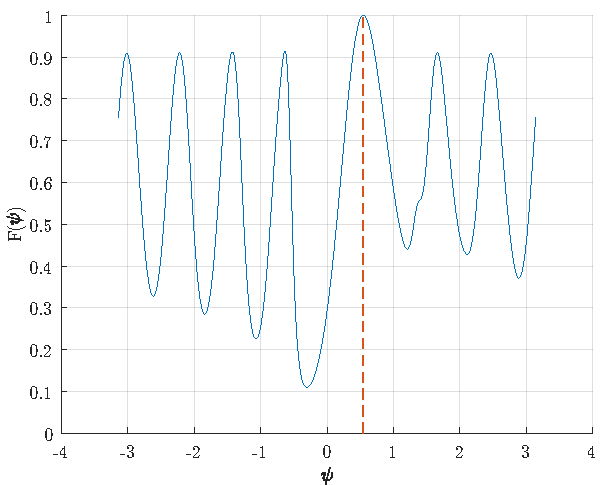
\includegraphics[width=\linewidth]{figs/fig4.10a}
        \caption{}
        \label{fig:4.10a}
    \end{subfigure}
    \begin{subfigure}{0.49\linewidth}
        \centering
        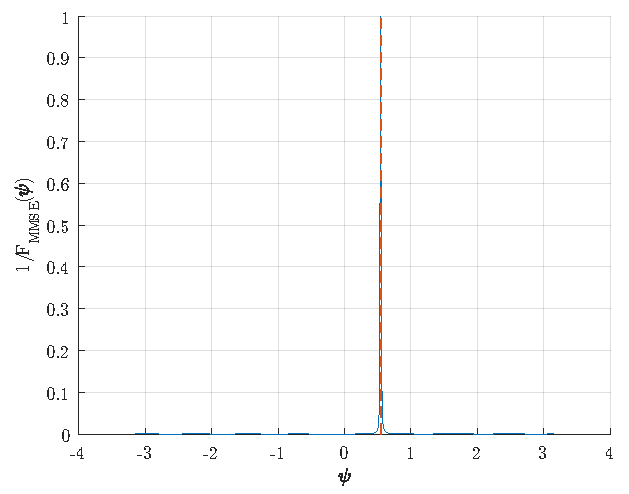
\includegraphics[width=\linewidth]{figs/fig4.10b}
        \caption{}
        \label{fig:4.10b}
    \end{subfigure}
    \caption{ \subref{fig:4.11a} Инверсная нормированная $F_{MMSE}(\psi)$, \subref{fig:4.11b} нормированная $F(\psi)$, $\psi=10^\circ(\psi \approx 0.55), \text{SNR}=30$ дБ}
\end{figure}

Прямое вычисление $F(\psi)$ и поиск его максимума ведет к большим вычислительным затратам. Можно применить условие $F'(\psi) =0$ и получить следующее условие
\begin{equation}
    \label{eq:4.31}
    \begin{aligned}
        \mu(\psi) = &
        \qty(\sum\limits_m f'_m(\psi) \hat p_m) \qty(\sum\limits_m f^2_m(\psi))                              \\
                    & - \qty(\sum\limits_m f_m(\psi)\hat p_m) \qty(\sum\limits_m f_m (\psi) f'_m(\psi)) = 0,
    \end{aligned}
\end{equation}
\begin{equation}
    \label{eq:4.32}
    \begin{aligned}
        f'_m(\psi) = \frac{\sin(0.5N (\psi - \chi_m))}{2\sin^3(0.5(\psi - \chi_m))} \times
        \big[
          & (N-1)\sin(0.5(N+1) (\psi - \chi_m)) - \\
        - & (N+1) \sin(0.5(N-1)(\psi - \chi_m))
            \big]
    \end{aligned}
\end{equation}
Типичный график $\mu(\psi)$ представлен на рис. \ref{fig:4.11}. Можно заметить, что вокруг заданного $\psi \approx 0.55$ (красная вертикальная линия) есть область где
$\mu(\psi)$ положительна слева и отрицательна справа. Поэтому, если известна грубая оценка угла прихода,
что и происходит на первом этапе алгоритма),
можно методом дихотомии быстро найти AOA с машинной точностью.
\begin{figure}[ht]
    \centering
    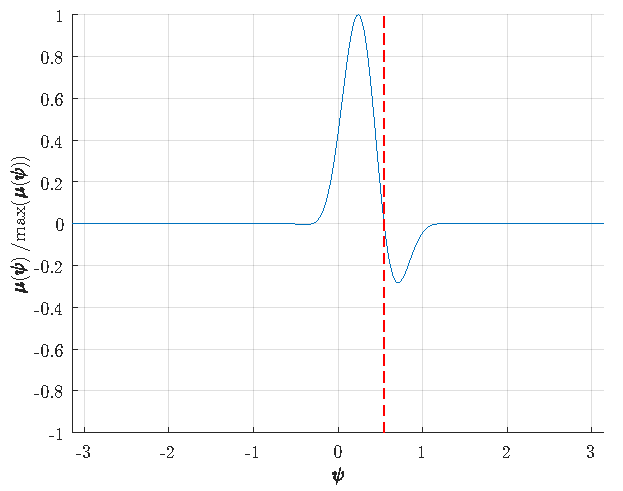
\includegraphics[width=0.75\linewidth]{figs/fig4.11}
    \caption{Нормированная функции $\mu(\psi)$, $\psi=10^{\circ} (\psi \approx 0.55), SNR=30$ дБ}
    \label{fig:4.12}
\end{figure}

\begin{algorithm}
    \caption{Метод дихотомии для оценки угла прихода для улучшенного алгоритма иерархического поиска (hSearchMMSE)}
    \label{lst:4.1}
    \begin{algorithmic}
        \State $\psi_{left} = \psi_{min}$
        \State $\psi_{right} = \psi_{max}$
        \State $\psi_{old} = \psi_{min}$
        \State $\Delta \psi = \infty$
        \While{$\Delta \psi > \epsilon$}
        \State $\hat \psi = 0.5 (\psi_{left} + \psi_{right})$
        \If{$\mu(\psi) < 0$}
        \State $\psi_{right} = \hat\psi$
        \Else
        \State $\psi_{left} = \hat\psi$
        \EndIf
        \State $\Delta \psi = \abs{\hat \psi - \psi_{old}}$
        \EndWhile
        \State \Return $0.5(\psi_{left} + \psi_{right})$
    \end{algorithmic}
\end{algorithm}

Заметим, что лучи вокруг фактического направления АОА вносят основной вклад в
\eqref{eq:4.30}, потому что они имеют более высокие веса. Таким образом, мы
можем рассматривать только лучи, измеренные на этапе процедуры уточнения, и
лучший луч, выбранный на этапе полного перебора. Кроме того, для
процедуры поиска желательно, чтобы фактический угол прихода находился в середине
рассматриваемых направлений лучей. Таким образом, мы должны модифицировать
процедуру измерения на этапе дополнительных измерений. Некоторые примеры
представлены на рис.  \ref{fig:4.12}.
Сплошными серыми линиями показаны ДН лучей, формируемые на первом этапе оценки.
(полного перебора). Сплошная красная линия -- ДН лучшего луча,
выбранного на первой стадии. Штриховые линии — ДН лучей на этапе
уточнения. Наконец, лучи, используемые в \eqref{eq:4.31}, отмечены цветными кривыми.

Всего, мы имеем два случая. В первом случае фактический угол прихода лежит
вблизи лучшего луча и мы проводим дополнительные измерения вокруг этого луча.
Во втором случае фактический угол прихода лежит посередине между лучшим и соседним
лучами. Следовательно, нам необходимо провести дополнительные измерения между ними.
В этом случае весовые векторы  формируются с помощью выражений \eqref{eq:4.19} и \eqref{eq:4.33}.
Знак в \eqref{eq:4.30} зависит от положения лучшего соседнего луча (слева или справа).
\begin{figure}[ht]
    \centering
    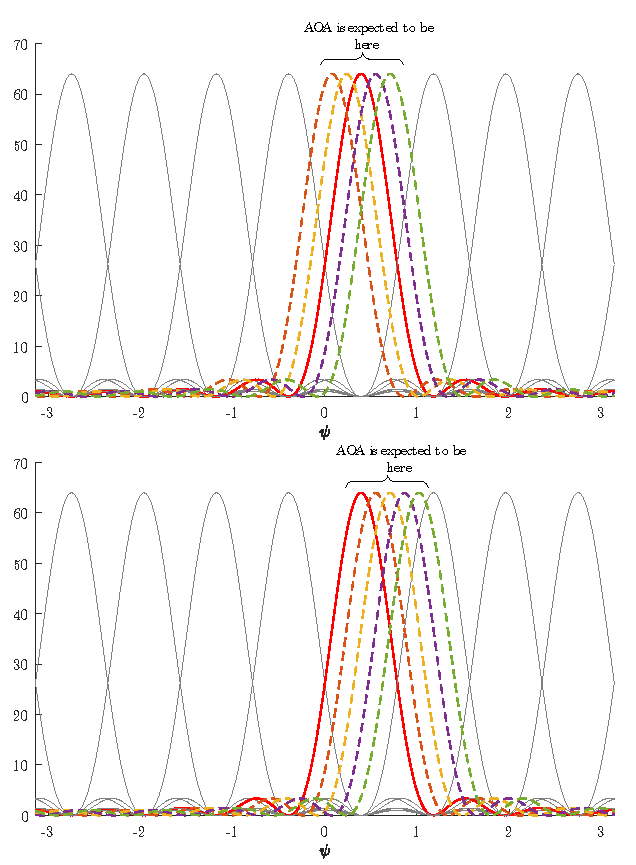
\includegraphics{figs/fig4.12}
    \caption{}
    \label{fig:4.12}
\end{figure}

\begin{equation}
    \label{eq:4.33}
    \chi_q = \eta_v \pm 2\pi \frac{q}{N(M+1)}; ~ q = 1 \dots M.
\end{equation}


Вопрос в том, как мы можем определить, где находится фактический угол прихода до этапа дополнительных измерений.
Предлагается использовать метрику \eqref{eq:4.30} для проверки трех гипотез:
\begin{itemize}
    \item $H_1$ -- угол прихода находится между лучшим лучем и левым соседним лучом
    \item $H_2$ -- угол прихода находится вблизи лучшего луча
    \item $H_3$ -- угол прихода находится между лучшим лучем и правым соседним лучом
\end{itemize}

\begin{figure}[ht]
    \centering
    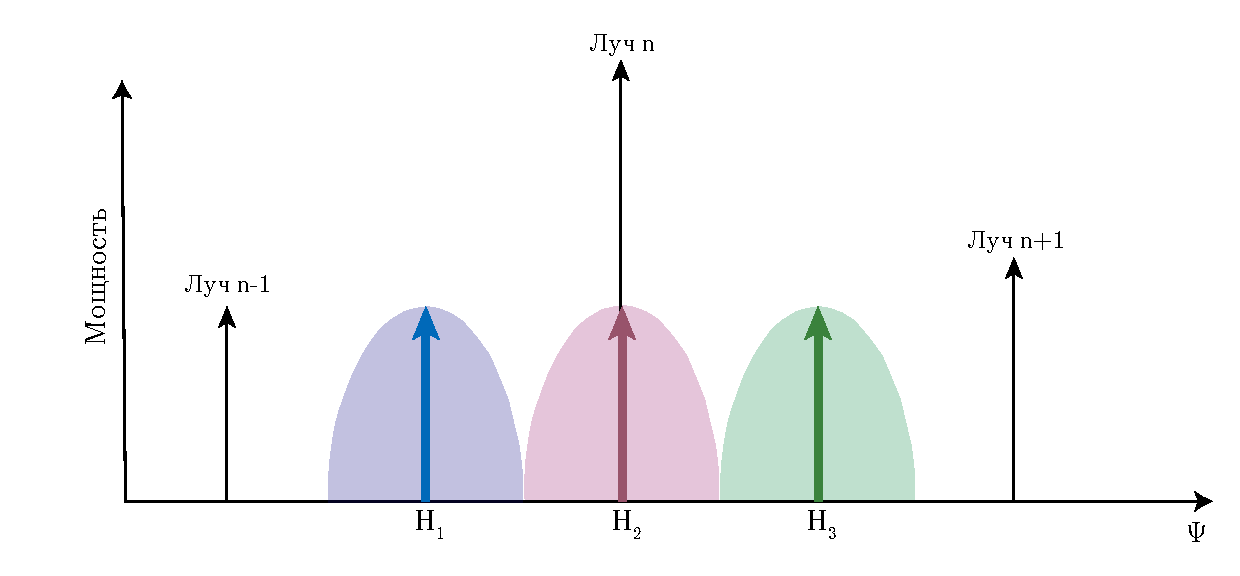
\includegraphics[width=0.75\linewidth]{figs/fig4.13}
    \caption{Выбор гипотез перед дополнительными измерениями. Черные стрелки принадлежат лучам из первой стадии прозвонки, цветные стрелки показываю центральные направления для различных гипотез}
    \label{fig:4.13}
\end{figure}

Если $\eta_v$ --  пространственная частота наилучшего луча на этапе основных измерений, выбранная нами метрика будет равна
\begin{equation}
    \label{eq:4.34}
    F_{H_n} = \qty[\sum\limits_{m=v-1}^{v+1} f_m (\psi_{H_n}) \hat p_m]^2 \qty[\sum\limits_{m=v-1}^{v+1}f_m^2(\psi_{H_n})]^{-1}
\end{equation}
\begin{equation}
    \label{eq:4.35}
    f_m(\psi_{H_n}) = \frac{\sin^2 (0.5N(\psi_{H_n} - \eta_{m}))}{\sin^2(0.5(\psi_{H_n} - \eta_{m}))}.
\end{equation}
\begin{equation}
    \label{eq:4.36}
    \begin{matrix}
        \psi_{H_1} = \frac{\eta_{v-1} + \eta_v}{2}; &
        \psi_{H_2} = \eta_{v}                       &
        \psi_{H_1} = \frac{\eta_{v+1} + \eta_v}{2}; &
    \end{matrix}
\end{equation}


Тогда структурная схема алгоритма будет следующей
\begin{enumerate}[label=\textbf{Шаг \arabic*:}]
    \item Этап полного перебора. BS производит сканирование лучом, UE
          последовательно использует все лучи из своей кодовой книги \eqref{eq:4.16} для
          измерения мощности на каждом луче BS. Процедура выполняется для обоих АР.
    \item Выбирается лучшая пара лучей UE-BS и рассматривается выбранный луч UE
          как лучший сектор с пространственной частотой $\eta_v$.
    \item Проверяются гипотезы $H_1, H_2$ и $H_3$ (см. \ref{fig:4.13}) используя метрику \eqref{4:34}.
          Выбирается гипотеза с наибольшим значением метрики. Отметим, что если в
          качестве лучшего луча выбирается первый луч UE ($v=1$), то гипотеза
          $H_1$ не тестируется.
          Аналогично, не тестируется гипотеза $H_3$ для последнего луча с
          индексом $v=8$.  \item  Этап дополнительных измерений. BS также
          производит сканирование лучом.  UE последовательно использует все лучи
          из кодовой книги \eqref{eq:4.19} для измерения мощности на каждом луче
          BS. Если выбрана гипотеза $H_2$, для формирования кодовой книги
          используется \eqref{eq:4.20}.  В остальных случаях используется
          \eqref{eq:4.33}. Знак <<$-$>> соответствует $H_1$, а <<$+$>>
          соответствует  $H_3$.
    \item Выполняется алгоритм поиска Алг. \ref{lst:4.1}, используя условие МСКО
          \eqref{eq:4.31}. В уравнение подставляется мощность лучшего луча, измеренная
          на шаге 2 и мощность лучей из шага 4. Луч BS выбирается таким же, как в
          лучшей паре на шаге 2.
    \item Рассчитывается угол прихода $\hat \phi$ на основе предполагаемой
          пространственной частоты. Если лучшая пара лучей UE-BS относится к АР\#1, то
          $\hat \phi_{AOA} = \hat \phi$. Если лучшая пара UE-BS относится к AР\#2, то
          $\hat \phi_{AOA} = \hat \phi + \pi$.
\end{enumerate}


Временн\'{а}я структура алгоритма иерархического поиска с минимизацией
среднеквадратичной ошибки (\textit{hSearchMMSE}) представлена на рис. \ref{fig:4.9}.
Параметры алгоритма представлены в таб. \ref{tab:4.3}.
\begin{table}
    \centering
    \caption{Параметры алгоритма hSearchMMSE}
    \label{tab:4.3}
    \begin{tabular}{|l|c|}
        \hline
        Параметр                             & SS burst  \\
        \hline
        N / M / AIPs                         & 8 / 4 / 2 \\
        Число просканированных лучей (UE/BS) & 20 / 64   \\
        Суммарное число RS                   & 1280      \\
        Необходимое время (слот 0.125 мс)    & 384 мс    \\
        \hline
    \end{tabular}
\end{table}

\subsection{Модифицированный алгоритм моноимпульса}
Идея алгоритма основанного на монопульсе, также известного как \textit{Auxiliary Beam}, была
предложена в \cite{Zhu2016} и \cite{Kim2019}. В отличие от обычных алгоритмов
монопульса (см. раздел \ref{sec:monopulse}), AuxBeam основан на мощности и не
требует сложного измерения амплитуды. Кроме того, для зондирования требуется
достаточно малое количество лучей, и он совместим с алгоритмами слежения. 

Основная идея в следующем. Пусть $\eta_u$ и $\eta_{u+1}$ -- обобщенные углы
лучей такие, что $\eta_u<\psi<\eta_{u+1}$ (см. рис. \ref{fig:4.14}), где $\psi$
-- обобщенный угол прихода волны.  Пусть $\eta_{u+1}$ ортогонален $\eta_u$, то
есть $\eta_{u+1} = \eta_u + 2\delta$, где $\delta = \pi/N$  и $\tilde \eta_u =
0.5 (\eta_u + \eta_{u+1})$ -- центральное направление.
\begin{figure}[ht]
    \centering
    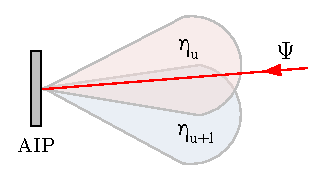
\includegraphics[width=0.5\linewidth]{figs/fig4.14}
    \caption{Конфигурация лучей для AuxBeam}
    \label{fig:4.14}
\end{figure}
Тогда можно рассмотреть следующую метрику, однозначно зависящую от угла прихода
\begin{equation}
    \label{eq:4.37}
    \zeta(\psi) = \frac{f_u(\psi) - f_{u+1}(\psi)}{f_u(\psi) + f_{u+1}(\psi)} = - \frac{\sin(\psi - \tilde \eta_u) \sin \delta}{1 - \cos(\psi - \tilde \eta_u) \cos \delta}
\end{equation}
\begin{equation}
    \label{eq:4.38}
    f_u(\psi) = \frac{\sin^2 (0.5 N (\psi - \eta_u))}{\sin^2(0.5 (\psi - \eta_u))}
\end{equation}
Зависимость метрики $\zeta(\psi)$  от обобщенного угла прихода представлена на
рис. \ref{fig:4.15}.
\begin{figure}[ht]
    \centering
    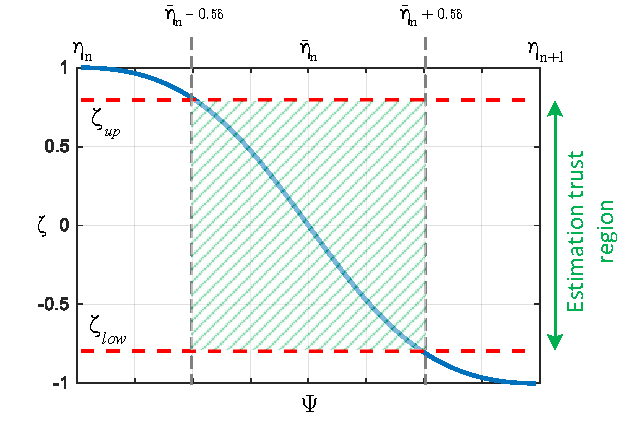
\includegraphics[width=0.5\linewidth]{figs/fig4.15}
    \caption{Зависимость метрики $\zeta(\psi)$ для алгоритма AuxBeam}
    \label{fig:4.15}
\end{figure}
В реальной системе метрика $\hat \zeta$ может быть оценена следующим образом
\begin{equation}
    \label{eq:4.39}
    \hat \zeta = \frac{\hat p_u - \hat p_{u+1}}{ \hat p_u + \hat p_{u+1} },
\end{equation}
где $\hat p_u$ -- мощость измеренная на $u$-ом луче. Эта оценка получается смещенной, поскольку $\hat p_u$ включает мощность шума.
Чтобы избежать этого, в знаменателе можно вычесть удвоенную мощность шума, но это может обратить метрику в бесконечность при малом SNR.
И, поскольку, функция $\zeta(\psi)$ достаточно полога на краях интервала $(\eta_u, \eta_{u+1})$, это приводит к высокому
воздействию шума на метрику при вычислении обратной функции.

Кроме того, если угол прихода находится рядом с центральным направлением определенного
луча, мы можем выбрать другой луч так, что условие $\eta_u<\psi < \eta_{u+1}$ не будет выполняться.
Чтобы этого не произошло, предлагается ввести условие на доверительный интервал
$\zeta_{low}<\hat \zeta < \zeta_{up}$, который изображен зеленой штриховкой  на рис.
\ref{fig:4.15}.

Если условие доверительного интервала не выполняется, следует провести дополнительные измерения на смещенных лучах.
Если оно выполняется, можно оценить угол прихода как
\begin{equation}
    \label{eq:4.41}
    \hat \psi = \tilde \eta_u - \arcsin(
    \frac{\hat \zeta \sin\delta}{\sin^2\delta + \hat \zeta^2 \cos^2\delta} -
    \frac{\hat \zeta \sqrt{1- \hat \zeta^2} \sin\delta\ \cos\delta}{\sin^2\delta + \hat \zeta^2 \cos^2\delta}
    )
\end{equation}
\begin{enumerate}[label=\textbf{Шаг \arabic*:}]
    \item Этап сканирования. BS производит сканирование лучом, UE
          последовательно использует все лучи из кодовой книги \eqref{eq:4.16} и \eqref{eq:4.17} для
          измерения мощности на каждом луче BS. Процедура выполняется для обоих AIP.
    \item По результатам измерений, выбирается лучшая пара лучей UE-BS. Для того же луча BS,
          выбирается самый сильный сосед, первого найденного луча. Используя измеренную мощность для выбранных лучей
          вычисляется метрика \eqref{eq:4.39}. Пример выбранных лучей UE представлен на рис. \ref{eq:4.16}.
    \item Если условие $\zeta_{low} < \hat \zeta < \zeta_{up}$, выполняется оценка обобщенного угла прихода $\hat \psi$ используя \eqref{eq:4.41} и пропускается шаг 4.
    \item Пусть $\eta_v$ -- обобщенный угол лучшего луча UE. Проводятся измерения на обобщенных углах
          $\eta_{v+0.5} = \eta_v - \delta$ и
          $\eta_{v-0.5} = \eta_v + \delta$. Дополнительные лучи показаны на рис. \ref{fig:4.16} пунктирными линиями. Далее вычисляется метрика \eqref{eq:4.39}
          и оценивается обобщенный угол прихода $\hat \psi$ (см. \eqref{eq:4.41}).
    \item Рассчитывается угол прихода $\hat \phi$ на основе предполагаемой пространственной частоты. Если лучшая пара лучей UE-BS
          относится к AIP1, то $\hat \phi_{AOA} = \hat \phi$. Если лучшая пара UE-BS относится к AIP2, то $\hat \phi_{AOA} = \hat \phi + \pi$.
\end{enumerate}

\begin{figure}[ht]
    \centering
    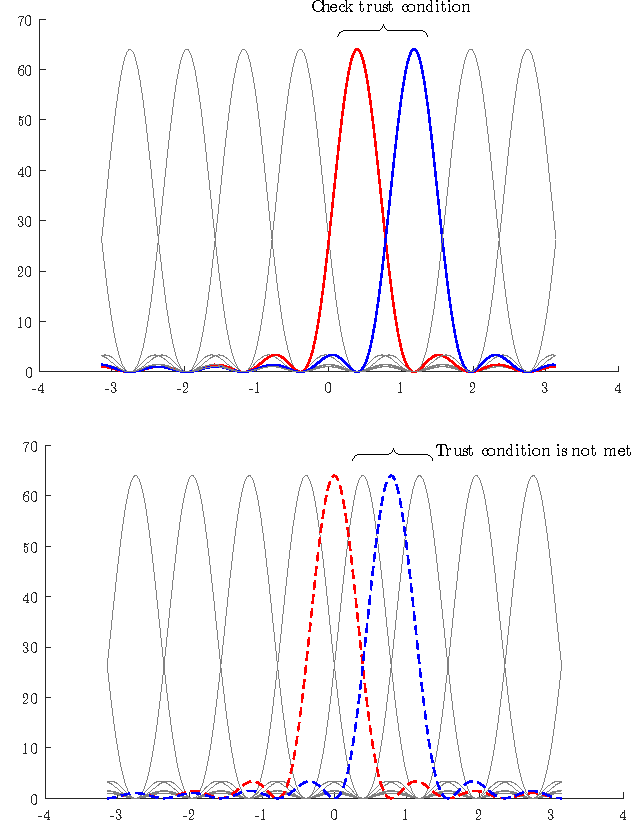
\includegraphics{figs/fig4.16}
    \caption{Два варианта выбора лучей UE для алгоритма AuxBeam. Верхний -- в случае выполнения условия на доверительный интервал, нижний -- в обратном случае.}
    \label{<label>}
\end{figure}


\begin{figure}[ht]
    \centering
    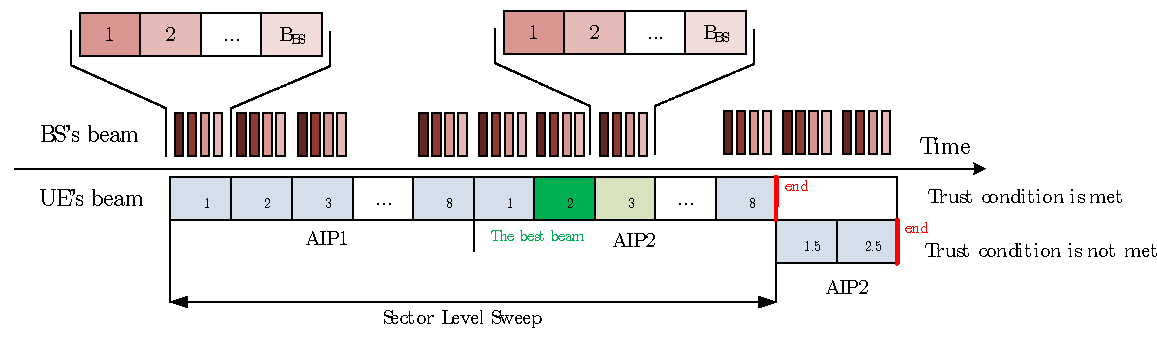
\includegraphics[width=\linewidth]{figs/fig4.17}
    \caption{Изображение процедуры иерархического поиска (baseline) во времени для двух антенных решеток. $N=8$, $M=4$, 64 луча BS}
    \label{fig:4.9}
\end{figure}

Временн\'{а}я структура алгоритма AuxBeam представлена на рис. \ref{fig:4.17}. Параметры алгоритма представлены в таб. \ref{tab:4.4}.
\begin{table}
    \centering
    \caption{Параметры алгоритма AuxBeam}
    \label{tab:4.3}
    \begin{tabular}{|l|c|}
        \hline
        Параметр                             & SS burst        \\
        \hline
        N / M / AIPs                         & 8 / 0 или 2 / 2 \\
        Число просканированных лучей (UE/BS) & 16 или 18 / 64  \\
        Суммарное число RS                   & 1024 или 1152   \\
        Необходимое время (слот 0.125 мс)    & 304 или 344 мс  \\
        \hline
    \end{tabular}
\end{table}

\subsection{Сканирование адаптивным методом бисекций}

Еще один многообещающий метод —  Compressed Sensing Algrorithm, идея которого описана \cite{Alkhateeb2014}.
Базовая концепция следующая. Пусть имеется сетка возможных
обощенных углов прихода волны $\psi_q = - \pi\frac{(Q-1)}{Q} + \frac{2\pi}{Q} (q-1)$, где $Q$ -- размер сетки.
Мы можем представить сигнал, измеренный пользователем (UE) для фиксированного
луча BS, как
\begin{equation}
    \label{eq:4.42}
    y = \vec w^H\vec S \vec a + \vec \xi,
\end{equation}
\begin{equation}
    \label{eq:4.43}
    \vec S =
    \begin{bmatrix}
        \vec s(\psi_1) & \vec s(\psi_2) & \dots & \vec s(\psi_q) \\
    \end{bmatrix},
\end{equation}
\begin{equation}
    \label{eq:4.44}
    \vec s =
    \begin{bmatrix}
        1 & \exp{i\psi} & \dots & \exp\{ i(N-1)\psi\} \\
    \end{bmatrix}^T,
\end{equation}
\begin{equation}
    \label{eq:4.45}
    \vec a =
    \begin{bmatrix}
        0 & \dots & 0 & a & 0 & \dots 0 \\
    \end{bmatrix}^T,
\end{equation}

где $\vec w$ -- весовой вектор пользователя,
$\vec s(\psi)$ -- диаграмообразующий вектор,
$N$ -- число элементов в антенной решетке,
$\vec \xi$ -- вектор шума,
$\vec z$ -- вектор комплексной аплитуды размерности $(Q\times 1)$,
где все элементы нулевые, кроме одного, отвечающему фактическому углу
прихода излучения на решетку.
Основная задача алгоритмов этого семейства -- восстановить вектор $\vec a$
используя количество измерений $L \ll Q$.  Если мы рассмотрим некоторую кодовую
книгу $\vec W$ размером $(N \times L)$, чьи столбцы являются весовыми векторами
для луча пользователя, результат сканирования будет
следующим
\begin{equation}
    \label{eq:4.46}
    y = \vec W^H\vec S \vec a + \vec \xi,
\end{equation}

В работе \cite{Alkhateeb2014}, авторы утверждают, что их адаптивный алгоритм более эфективен,
чем обычный алгоритм бисекции. В адаптивном алгоритме процедура зондирования разбита на несколько этапов
и кодовая книга $\vec W$ текущего этапа зависит от предыдущих результатов. Понятно, что если нас не интересует значение $a$, то
вектор $\vec a$ может быть сжат до вектора $\vec z$. Этот вектор кодирует позицию ненулевого жлемента в векторе $\vec a$ (индекс $q$) и
требует только $\log(Q)$ итераций.

На первом шаге считаем, что ненулевой жлемент имеет индекс от $1$ до $Q/2$ ($z_1=0$) или
$Q/2+1$ до $Q$ ($z_1=1$). Для этого нам необходимо сформировать кодовую книгу $\vec W$ размерности $(N \times 2)$, которая удовлетворяет условию
\begin{equation}
    \label{eq:4.47}
    \vec S^H \vec W = \alpha \vec G,
\end{equation}
\begin{equation}
    \label{eq:4.48}
    \vec G =
    \begin{pmatrix}
        1 & \dots & 1 & 0 & \dots & 0 \\
        0 & \dots & 0 & 1 & \dots & 1 \\
    \end{pmatrix}^T,
\end{equation}
где $\vec G$ -- матрица $(Q \times 2)$ и $\alpha$ -- нормировочный множитель.
Физически это означает, что первый весовой вектор должен обеспечивать однородную структуру ДН по
обобщенным углам $\psi_1 \dots \psi_{Q/2}$ и подавлять ДН в направлениях $\psi_{Q/2 + 1}\dots \psi_Q$. Второй весовой вектор должен сделать противоположное.
Приближенное решения для кодовой книги $\vec W$ получается следующим
\begin{equation}
    \label{eq:4.49}
    \vec W = \alpha (\vec S \vec S^H)^{-1} \vec S \vec G
\end{equation}

\begin{figure}[ht]
    \centering
    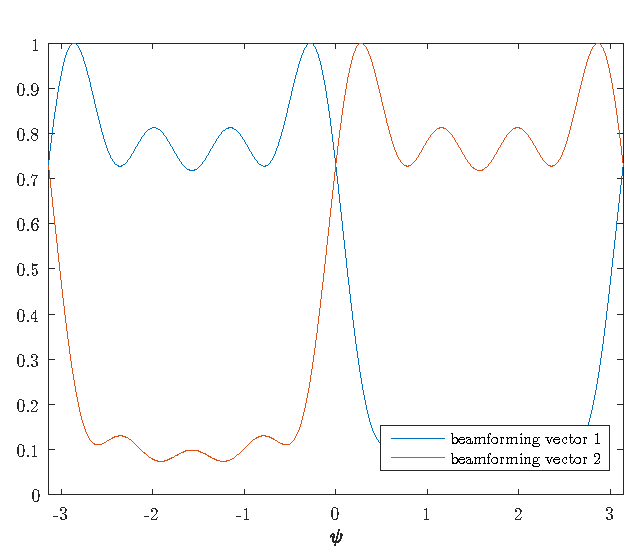
\includegraphics[width=0.5\linewidth]{figs/fig4.18}
    \caption{ДН для первого шага алгоритма $Q=40,~N=8$}
    \label{fig:4.18}
\end{figure}
Кодовый вектор, при котором будет принята наибольшая мощность будет соответствовать
первому приближению направления на источник. Пусть $z_1 = 0$. Тогда на следующим шаге
мы должны определить $z_2$. Это означает, что ненулевой элемент лежит между индексами $1$ или $Q/4$ ($z_2 =0 | z_1 =0$) или
между ииндексами $Q/4 + 1$ и $Q/2$ ($z_1 = 1 | z_1 = 0$). В этом случае матрица $\vec G$ определяется как
\begin{equation}
    \label{eq:4.48}
    \vec G =
    \begin{pmatrix}
        1 & \dots & 1 & 0 & \dots & 0 & 0 & \dots & 0 & 0 & \dots & 0 \\
        0 & \dots & 0 & 1 & \dots & 1 & 0 & \dots & 0 & 0 & \dots & 0 \\
    \end{pmatrix}^T.
\end{equation}
\begin{figure}[ht]
    \centering
    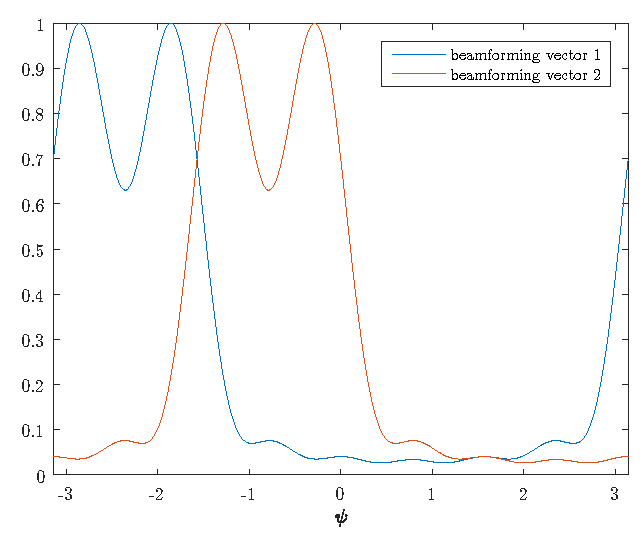
\includegraphics[width=0.5\linewidth]{figs/fig4.19}
    \caption{ДН для второго шага алгоритма, если $z_1=0$, $Q=40,~N=8$}
    \label{fig:4.19}
\end{figure}

Таким образом, ненулевые элементы в матрице $\vec G$ определяются сканированием необходимого индекса луча.
Процедура продолжается до тех пор, пока не будет определен последний элемент $z$. Проблема в том, что
с выбранной в данной работе аппаратной конфигурации пользователя мы не можем
применить \eqref{eq:4.49}, поскольку у нас не хватает степеней свободы, чтобы
обеспечить равномерное формирование направленности в одной области пространства
и полностью подавить други. Поэтому, мы предлагаем некоторую модификацию этого алгоритма на основе дихотомии, следуя физическим принципам вышеизложенного.

\begin{enumerate}[label=\textbf{Шаг \arabic*:}]
    \item BS периодически переключает свои лучи, UE использует следующий весовой вектор $\vec w = \mqty*[1 & 0 & \dots & 0]^T$ для каждой AIP.
          Физически это означает, что отключаются все элементы АР, кроме одного. ДН всей решетки совпадает с ДН элемента и становится квази-всенаправленной.
          Выбирается та AIP, где результирующая измеренная мощность оказывается больше.
    \item BS периодически переключает свои лучи. Обозначим $\eta_{left} = - \pi$, $\eta_{right} = + \pi$.
          На стороне пользователя применяется следующая кодовая книга
          \begin{equation}
              \vec W =
              \begin{pmatrix}
                  \mqty{ 1 & \exp{i\eta_1}} & \zmat{1}{6} \\
                  \mqty{ 1 & \exp{i\eta_2}} & \zmat{1}{6} \\
              \end{pmatrix}
          \end{equation}
          \begin{equation}
              \eta_1 = \frac34 \eta_{left} + \frac14 \eta_{right}; ~ \eta_2 = \frac14 \eta_{left} + \frac34 \eta_{right}
          \end{equation}
          Если первый вектор бимформинга обеспечил наибольшую принятую мощность, то
          $\eta_{right} = 0.5 (\eta_{left} + \eta_{right})$.
          В другом случае
          $\eta_{left} = 0.5 (\eta_{left} + \eta_{right})$.
          \begin{figure}[h!]
              \centering
              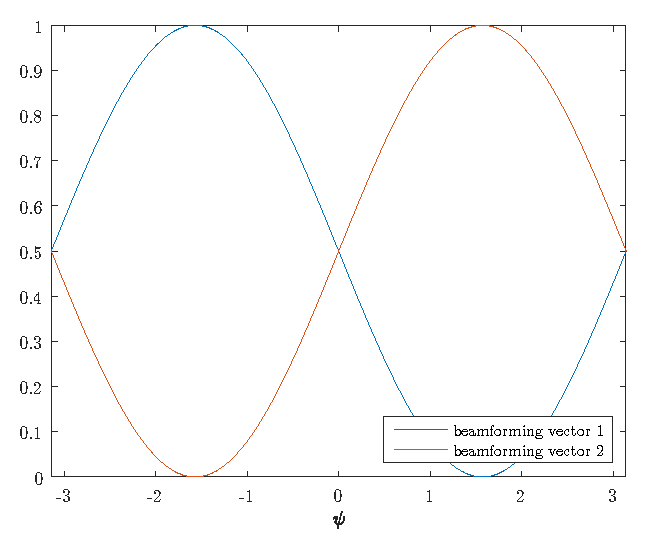
\includegraphics[width=0.5\linewidth]{figs/fig4.20}
              \caption{}
              \label{fig:4.20}
          \end{figure}
    \item BS периодически переключает свои лучи. Пользователь использует следующую кодовую книгу
          \begin{equation}
              \vec W =
              \begin{pmatrix}
                  \mqty{ 1 & \exp{i\eta_1} & \exp{i2\eta_1} & \exp{3i\eta_1}} & \zmat{1}{4} \\
                  \mqty{ 1 & \exp{i\eta_2} & \exp{i2\eta_2} & \exp{3i\eta_2}} & \zmat{1}{4} \\
              \end{pmatrix}
          \end{equation}
          \begin{equation}
              \eta_1 = \frac34 \eta_{left} + \frac14 \eta_{right}, ~ \eta_2 = \frac14 \eta_{left} + \frac34 \eta_{right}
          \end{equation}
          \begin{figure}[h!]
              \centering
              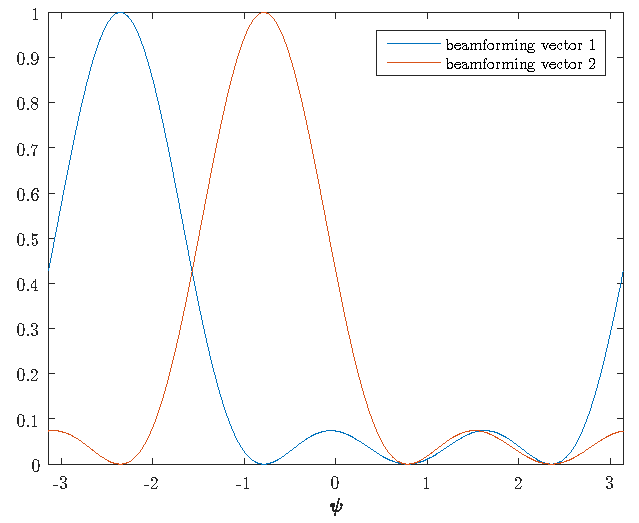
\includegraphics[width=0.5\linewidth]{figs/fig4.21}
              \caption{}
              \label{fig:4.21}
          \end{figure}
          Если первый вектор бимформинга обеспечил наибольшую принятую мощность, то
          $\eta_{right} = 0.5 (\eta_{left} + \eta_{right})$.
          В другом случае
          $\eta_{left} = 0.5 (\eta_{left} + \eta_{right})$.
    \item BS периодически переключает свои лучи. Пользователь использует следующую кодовую книгу
          \begin{equation}
              \vec W =
              \begin{pmatrix}
                  1 & \exp{i\eta_1} & \exp{i2\eta_1} & \dots & \exp{i(N-1)\eta_1} \\
                  1 & \exp{i\eta_2} & \exp{i2\eta_2} & \dots & \exp{i(N-1)\eta_2}
              \end{pmatrix}
          \end{equation}
          \begin{equation}
              \eta_1 = \frac34 \eta_{left} + \frac14 \eta_{right}, ~ \eta_2 = \frac14 \eta_{left} + \frac34 \eta_{right}
          \end{equation}
          \begin{figure}[h!]
              \centering
              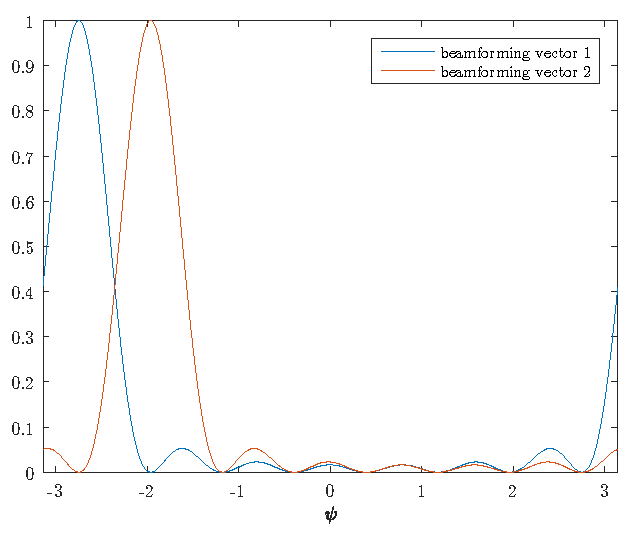
\includegraphics[width=0.5\linewidth]{figs/fig4.22}
              \caption{}
              \label{fig:4.22}
          \end{figure}
          Если первый вектор бимформинга обеспечил наибольшую принятую мощность, то
          $\eta_{right} = 0.5 (\eta_{left} + \eta_{right})$.
          В другом случае
          $\eta_{left} = 0.5 (\eta_{left} + \eta_{right})$.
    \item Предыдущий шаг повторяется, пока не достигнется желаемая точность. Отметим, что ширина ДН начиная с этого шага перестает меняться, изменяется тольно направление луча.
    \item Вычисляем угол прихода используя оцененный обобщенный угол $\hat \psi = 0.5 (\eta_{left} + \eta_{right})$. Если на шаге 1 была выбрана первая решетка, то
          $\hat \phi_{AOA} = \hat \phi$, в противном случае $\hat \phi_{AOA} = \hat \phi + \pi$.
\end{enumerate}

\begin{figure}[h!]
    \centering
    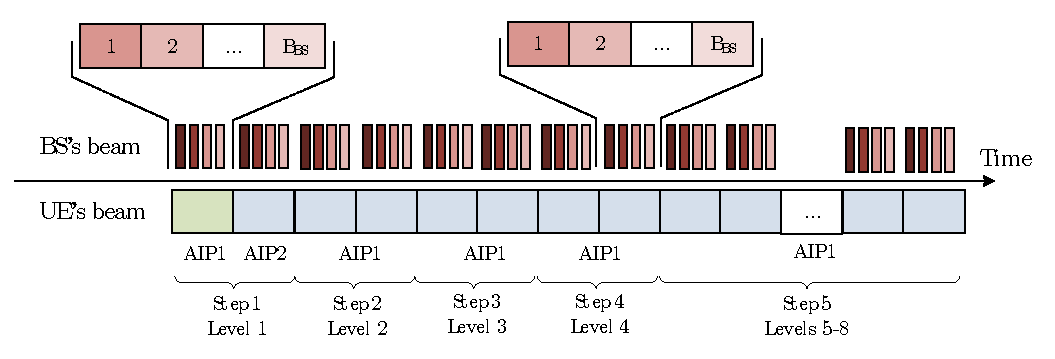
\includegraphics[width=0.5\linewidth]{figs/fig4.23}
    \caption{}
    \label{fig:4.23}
\end{figure}

